\chapter{Ecosistema e strumenti}
\label{ch:ecosistema}
In questo capitolo verranno descritti i linguaggi utilizzati e gli
strumenti impiegati nell'analisi, nello sviluppo e nei test della libreria.
Di ogni elemento verrà fornita una breve panoramica, ponendo
maggior enfasi sugli aspetti (alle volte piuttosto tecnici) che è
stato necessario tenere in considerazione durante lo sviluppo
di \pygfa.

\section{Il linguaggio Python}
\nocite{wiki-python}
Python è un linguaggio di programmazione ideato da Guido van Rossum
all'inizio degli anni `90. Python è un linguaggio che si appresta a molteplici
stili di programmazione, sfruttando caratteristiche del paradigma object
oriented, funzionale e della programmazione strutturata.
Tali proprietà permetto l'uso del linguaggio in una grande varietà di attività:
nella creazione di script di automazione di sistema, nella scrittura di
sistemi web di backend fino allo sviluppo di complesse librerie di analisi numerica
e machine learning.

\begin{wrapfigure} {O} {0.35\textwidth}
	\begin{centering}	
		
\includegraphics{python-logo}
		\caption[Logo Python]{Logo del linguaggio di programmazione Python.}
	\end{centering}
\end{wrapfigure}
La minima struttura necessaria a produrre un programma Python,
l'inferenza del tipo delle variabili a runtime (\emph{dynamic typing}),
la gestione automatica della memoria e la sua espressività lo rendono
un candidato ideale nella prototipazione di sistemi nuovi, coerente con
processi di sviluppo agili e con la pratica di extreme programming.

Inoltre Python è un linguaggio interpretato, di conseguenza è possibile
effettuare, direttamente all'interno dell'interprete, verifiche in tempo
reale delle funzionalità attualmente in sviluppo.
Il fatto che il linguaggio venga interpretato
da un interprete permette una facile integrazione del codice nativo
con il quale l'interprete stesso è stato implementato.
Per questo motivo -e grazie al livello di astrazione sul quale si colloca-
esistono diverse implementazioni del linguaggio Python
che sfruttano la JVM, la piattaforma .NET, il linguaggio C o che si
concentrano maggiormente su alcuni aspetti specifici come la velocità,
il multithreading e la minimalità per l'uso in ambienti embedded.

\captionsetup{justification=centering, singlelinecheck=false}
\begin{lstlisting}[language=Python, frame=topline, caption=Un esempio  dell'espressività\\del linguaggio applicata a \pygfa.]
>>> import pygfa
>>> gfa = pygfa.gfa.GFA.from_file("data/sample1.gfa")
>>> gfa.nodes()
['1', '3', '2', '5', '13', '6', '11', '12', '4']
>>> pygfa.nodes_connected_components(gfa) #calcola i nodi
	di ciascuna componente connessa
...
[{'2', '1', '3', '6', '5'}, {'11', '13', '12'}, {'4'}]
>>> # estrai tutte le componenti connesse
	con numero di nodi maggiore di 3
...
>>> [component for component in pygfa.nodes_connected_components(gfa)
	if len(component) > 3]
[{'2', '1', '3', '6', '5'}]
\end{lstlisting}
\captionsetup{justification=justified, singlelinecheck=false}

\subsection{Classi, convenzioni e duck typing}
In Python per creare una classe è necessario definirla mediante
la dicitura:
\begin{lstlisting}[language=Python]
class MiaClasse(Antenata1, Antenata2, ...):
	...
\end{lstlisting}
Come è possibile notare, è ammissibile ereditare da più classi.
Tale caratteristica non è molto frequente negli altri linguaggi e
viene spesso considerata una cattiva pratica, visto che non
permette di accorgersi di una errata definizione della gerarchia delle
classi di progetto. Tuttavia, in Python questa proprietà permette
l'aggiunta di funzionalità alla classe, in modo analogo alla modalità
\texttt{implements} di Java, rendendo possibile una definizione di
quelle che in realtà sono le interfacce e le loro implementazioni.
In \pygfa tale funzionalità è stata applicata per aggiungere le
funzionalità degli iteratori personalizzati alla classe \texttt{GFA}.

Python è un linguaggio fortemente influenzato dai movimenti
open source; infatti ogni programma, libreria e sistema scritto in Python
presuppone che l'utilizzatore abbia libero accesso al sorgente e che
possa capire le modalità di utilizzo di ogni modulo di cui è composto.
Per questo motivo i programmi tendono ad essere ricchi di documentazione,
sia essa incorporata nel codice che allegata nel manuale.
Come conseguenza il linguaggio non offre un meccanismo per definire i
metodi di una classe come privati; in virtù del fatto che l'utilizzatore, avendo
la piena possibilità di capire il funzionamento del singlo modulo di sistema,
ha la piena responsabilità delle sue azioni.
Per aiutare a distinguere elementi del programma che l'autore vorrebbe
fossero non utilizzati (o utilizzati con particolare consapevolezza) si è
soliti nominare tali elementi facendo precedere i loro nomi da un singolo
trattino basso (\emph{weak internal use}). E' possibile imprimere
maggior enfasi nell'oscuramento di un elemento precedendo
il suo nome da due trattini bassi, in tal modo l'accesso
all'elemento avviene precendo il nome della classe al nome dell'elemento.

\captionsetup{justification=centering}
\begin{lstlisting}[language=Python, frame=topline, caption=Convenzioni per l'uso interno.]
>>> class A:
...	def __init__(self):
...		self.normal_use = 5
...		self._internal_use = 10
...		self.__strong_internal = 15
...
>>> a = A()
>>> a.normal_use
5
>>> a._internal_use
10
>>> a._A__strong_internal
15
\end{lstlisting}
\captionsetup{justification=justified}

Una ulteriore convenzione comune al Python e ampiamente considerata
nello sviluppo di \pygfa è il cosiddetto \emph{duck typing}.
Visto che il Python usa il binding dinamico, le funzioni e i metodi non
possono verificare il tipo dei parametri passati tramite signature.
Una possibile soluzione è verificare il tipo del parametro mediante
la funzione \texttt{isinstance}, come avviene per esempio quando
si cerca di effettuare il \emph{downcast} dalla classe antenata
ad una sottoclasse nei linguaggi in cui il binding avviene staticamente.
Per esempio tale pratica si verifica in Java quando si va ridefinire il metodo
\texttt{equal} di una classe, avente come signature un tipo Object rappresentante
l'istanza da confrontare ed effettuando il downcasting del parametro alla classe
attuale prima di effettuare i confronti fra le due istanze.

In Python invece viene considerata un'altra via. L'oggetto passato come
parametro viene confrontato direttamente con l'istanza e in caso
di errori (per esempio l'oggetto potrebbe non avere un parametro al quale
si sta accedendo), viene lanciata un'eccezione dalla quale si ritorna l'ineguaglianza
fra i due oggetti. Questo è ciò che si intende per duck typing.

Questo comportamento permette di avere delle classi molto flessibili,
visto che la compatibilità fra le classi viene garantita dall'uguaglianza
delle interfacce (se due oggetti sono diversi, ma in un determinato
contesto hanno lo stesso comportamento, allora possono essere considerati
simili); ma potenzialmente annulla la simmetria dell'operatore d'uguaglianza.
Di conseguenza, dati due oggetti $A$ e $B$ di classi diverse, si può
avere la situazione in cui $A = B$, ma $B \neq A$.

\subsection{Perchè è stato scelto Python}
Oltre alle caratteristiche spiegate precedentemente che rendono Python
un linguaggio flessibile, potente e anche divertente da usare, altri fattori
che motivano la sua scelta sono:
\begin{itemize}
	\item l'elevato numero di librerie disponibili, di strumenti che accompagnano
		e velocizzano lo sviluppo e la manutenzione di un progetto:
		analizzatori di sintassi, strumenti di test e ambienti per la
		generazione automatica della documentazione;
	\item la sua diffusione in ogni campo di applicazione, compreso
		quello bioinformatico, che è una delle principali motivazioni dello sviluppo
		di \pygfa;
	\item l'ampia documentazione sia della libreria standard che delle librerie esterne,
		con soluzioni a buona parte dei problemi di programmazione comuni,
		comportando un abbassamento dei costi e dei tempi di manutenzione e
		sviluppo dei sistemi.
\end{itemize}

% NetworkX
\section{NetworkX}
NetworkX è una libreria Python che permette di creare e gestire grafi.
Essa fornisce inoltre un'ampia collezione di algoritmi applicabili a grafi e
alberi: algoritmi di attraversamento, di cammini minimi, di analisi del
flusso; sui quali si basa per fornire informazioni topologiche
del grafo, come la presenza di cicli, di componenti connesse e di
punti di articolazione.

La libreria usa le liste di adiacenza per rappresentare i nodi e gli archi ad essi
collegati mediante tre dizionari Python nidificati.
Il primo dizionario contiene gli identificativi univoci di ogni nodo e come valore
ha un secondo dizionario con chiavi i nodi collegati ad esso mediante un
arco. Il valore di questi è a loro volta un dizionario che rappresenta
gli archi che collegano il nodo del primo dizionario con quello definito nel secondo.

\begin{wrapfigure} {O} {0.35\textwidth}
	\begin{centering}	
		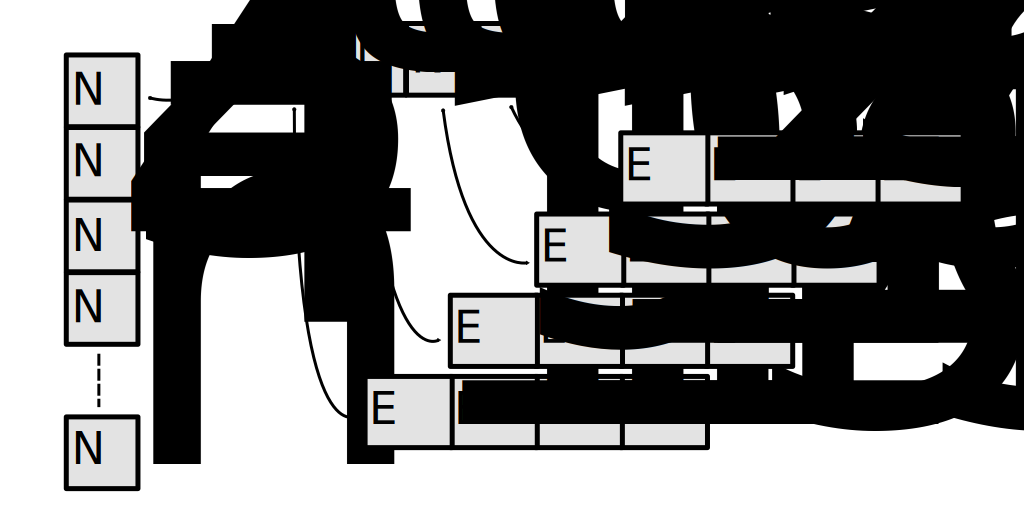
\includegraphics[scale=0.35]{networkx-dict}
		\caption[Rappresentazione nodi e archi networkx]{Rappresentazione grafica dei nodi e degli archi descritti in networkx.}
		\label{fig:networkx-dict}
	\end{centering}
\end{wrapfigure}

Questa scelta, oltre a rappresentare il modo più corretto per
implementare tale struttura\cite{python-graph}, permette un rapido
accesso ai nodi e agli archi che li mettono in relazione.

Oltre a specificare un identificativo univoco da assegnare a nodi e archi,
è possibile definire delle proprietà che possono essere dei tipi primitivi
o degli oggetti.

\subsection{Tipi di grafo}
Vi sono quattro differenti tipologie di grafo a disposizione:
\begin{itemize}
	\item grafo non diretto,
	\item grafo diretto,
	\item multigrafo non diretto,
	\item multigrafo diretto
\end{itemize}
Nel grafo non diretto, all'aggiunta di un arco $(u, v)$ tra
i nodi $u$ e $v$ viene aggiunto automaticamente un
arco $(v, u)$.

I multigrafi permettono di definire molteplici archi delimitati dalla
stessa coppia di nodi. In tal caso la definizione dell'identificativo
di un arco è di maggiore importanza, visto che sarà necessario
discriminare l'arco desiderato da un insieme di collegamenti
tra la stessa coppia di nodi. Per i multigrafi (diretti e non)
NetworkX permette, all'aggiunta di un arco, di specificare la chiave
(identificativo) associato all'arco che si sta inserendo; nel caso in cui
l'utente non definisce un identificativo, l'oggetto rappresentante il grafo
fornisce automaticamente un numero intero da assegnarli non ancora
utilizzato.

\subsection{Perchè è stata scelta e limiti}
\label{sec:nx-why-limits}
Il contenuto di un file GFA è direttamente rappresentabile mediante
un grafo, per questo sfruttare una libreria già esistente ha permesso
di velocizzare i tempi di sviluppo.

NetworkX offre la miglior implementazione dei grafi scritta in Python,
sfruttando dove richiesto librerie matematiche anche di basso livello
per garantire prestazioni molto alte in termini di velocità. La vasta
gamma di algoritmi a disposizione, uno sviluppo costantemente
attivo\cite{networkx-github} e un'ampia documentazione rendono
questa libreria un'ovvia candidata per lo sviluppo di \pygfa.

Uno svantaggio, dovuto all'implementazione direttamente in Python di
Networkx, è il consumo piuttosto elevato di memoria richiesto
per contenere il grafo. Tale peso è dovuto principalmente
all'uso dei dizionari come struttura di rappresentazione di nodi ed
archi. In \pygfa tale inconveniente è possibile notarlo specialmente
nei dizionari degli archi, che arrivano ad occupare più
di \SI{2}{\kilo\byte}.

Un altro aspetto negativo della libreria è che non permette l'impiego degli
algoritmi considerando le proprietà di archi e nodi. Ciò significa
che, supponendo di avere degli archi colorati (blu, giallo, rosso),
non è possibile applicare gli algoritmi solo agli archi di uno specifico
colore. Per questo in \pygfa si è reso necessario andare a ridefinire
(sfruttando il sorgente) gli algoritmi di interesse andando
a considerare nell'algoritmo i nodi definiti da un iteratore, che li
seleziona in base ad una proprietà dell'arco, evitando
di considerare l'intera lista di adiacenza del singolo nodo.

% Coverage.py
\section{unittest e Coverage.py}
Python è un linguaggio dinamico, per questo ogni
riga di un programma viene analizzata solo nel momento
in cui lo script viene lanciato. Ciò vuole significare che un errore
(esclusi quelli di sintassi) non può essere individuato prima
della sua esecuzione.

Per questo motivo nello sviluppo di \pygfa si è scelto di scrivere
i casi di test con la libreria \emph{unittest}, fornita direttamente
con l'interprete, e successivamente si sono andati ad analizzare
gli script dei casi di test con \emph{Coverage.py}.

Coverage.py è un programma Python in grado di misurare la
copertura del listato scritto, annotando le parti del codice che
sono state eseguite e creando un report (su file o su interfaccia web)
indicando le righe che necessitano ulteriore copertura.

Entrambi gli strumenti sono stati presi in considerazione per via
della loro facilità di integrazione nello sviluppo, per
la loro chiarezza nell'esposizione degli errori e delle statistiche
e per la loro diffusione tra gli sviluppatori.

\subsection{Funzionamento}
Lo strumento di analisi per la copertura prende in input un programma Python il quale
viene eseguito linea per linea. Tutti i file coinvolti nel programma
(poiché contenenti funzioni, classi o variabili usate presenti
nello script) vengono considerati nel calcolo della copertura. La
misura della copertura avviene sia per singolo file che sull'intero
insieme di file coinvolti dal programma. La copertura
sul singolo file viene calcolata come:
\begin{equation}
Cov(f) = \frac{\#linee_{coperte}}{\#linee_{totali}}
\end{equation}

unittest invece permette di confrontare il risultato di un'operazione rispetto
ad un valore atteso, fermando l'esecuzione nel caso in cui uno di questi
confronti fallisce. E' possibile inoltre confrontare il comportamento atteso
da una certa operazione, come l'invocazione di un'eccezione in caso di
operazioni non valide.

% Pylint
\section{Pylint}
\nocite{pylint}
Pylint è uno strumento di analisi del codice, curato dalla
Python Code Quality Authority\cite{pycqa}, in grado di applicare
una serie di regole atte a verificare:
\begin{itemize}
	\item la compatibilità del programma rispetto le convenzioni stabilite
		dal linguaggio\cite{python-pep8};
	\item problemi di importazione delle librerie;
	\item la presenza di variabili usate in un contesto in cui il loro valore
		sarebbe indefinito;
	\item il verificarsi di codice duplicato, sia all'interno dello stesso file
		sia fra sorgenti diverse.
\end{itemize}

Lo strumento quindi non solo fornisce dei meccanismi di standardizzazione
del codice, ma effettua quelle operazioni complementari a unittest e coverage.py
per la verifica della correttezza, da un punto di vista sintattico e simbolico,
del programma.

\subsection{Come è stato usato}

Pylint è uno strumento di \emph{controllo}, che fornisce suggerimenti riguardanti molti
aspetti del codice. Osservare tutti gli avvertimenti e risolvere tutti i problemi
rilevati avrebbe richiesto un prolungamento dei termini di consegna, oltre che
costituire un lavoro non prioritario.
Il suo impiego in \pygfa è voluto per cercare di uniformare una nuova libreria
Python con le convenzioni e le pratiche più comuni che la maggior parte degli
utilizzatori di questo linguaggio si aspettano, fornendo loro un ambiente
familiare nel quale la complessità non sia data dalla costante ricerca nella
documentazione di nomi e comportamenti insoliti circa elementi che compongono
la libreria. Generalmente si sono cercati di risolvere tutti quei problemi relativi gli standard
di nomenclatura oltre che problemi di analisi simbolica che avrebbero compromesso
il corretto funzionamento di \pygfa.

\addcontent{Indicare il numero di issue al momento della consegna di \pygfa.}

\section{Sphinx e Read the Docs}
\label{seq:sphinx-rtd}
Sphinx è uno strumento per la generazione automatizzata di documentazione
del codice. Grazie a questo strumento è possibile ricavare un manuale
ben formatto direttamente dal sorgente, il quale deve essere scritto
secondo un linguaggio ben specifico per indicare elementi di rilievo
del codice, come parametri, valori di ritorno, eccezioni,
note o link.

Sphinx è stato creato creato in origine per la documentazione ufficiale
del linguaggio Python\cite{python-doc} e fin da subito si è sparso
come strumento di aiuto nella documentazione di programmi scritti
non solo in questo linguaggio, ma anche in molti altri linguaggi supportati,
vista la sua flessibilità e i risultati ottimi che produce.

Esso usa il \emph{reStructuredText} come linguaggio di markup, permettendo
un'ampia espressività e una vasta gamma di notazioni come link (interni ed esterni),
definizione di tag personalizzati e liste (ordinate e non) oltre la possibilità
di scrivere formule matematiche in \LaTeX.

Sphinx permette di generare la documentazione finale nei formati più comuni:
HTML (con supporto mobile nativo), PDF e EPUB. Solitamente la scelta
più diffusa (che \pygfa segue) è quella di produrre la documentazione in
HTML e di renderla disponibile su \emph{Read the Docs}.

\phantomsection
\label{seq:sphinx}
Read the Docs è una piattaforma online, supportata dalla community,
appositamente pensata per salvare, catalogare e rendere disponibile
la documentazione scritta con Sphinx.
Il sito fornisce un ambiente Python e permette di collegare la documentazione
direttamente ad un repository di progetto su Github, evitando così di
dover mantenere aggiornate due copie di un singolo progetto separate.
Il sito usa l'ambiente Python per generare la documentazione di
progetto, permettendo di aggiungere le dipendenze del codice mediante
file di testo. La procedura è automatizzata (vedere figura
\ref{fig:rtd-build}) e il codice HTML risultante viene pubblicato sulla
piattaforma al termine del processo.

Grazie a Sphinx e Read the Docs è stato possibile documentare \pygfa
in modo facile e veloce, evitando di costruire soluzioni \emph{ad-hoc}
per la sua distribuzione e manutenzione e, allo tempo stesso,
si è riusciti ad ottenere un risultato più che accettabile utilizzando
i temi predisposti della piattaforma, garantendo all'utilizzatore
una facile consultazione sia da desktop che da mobile, una visione
del sorgente direttamente dalla documentazione e una funzione
di ricerca efficace.

\begin{figure}[h]
	\center
	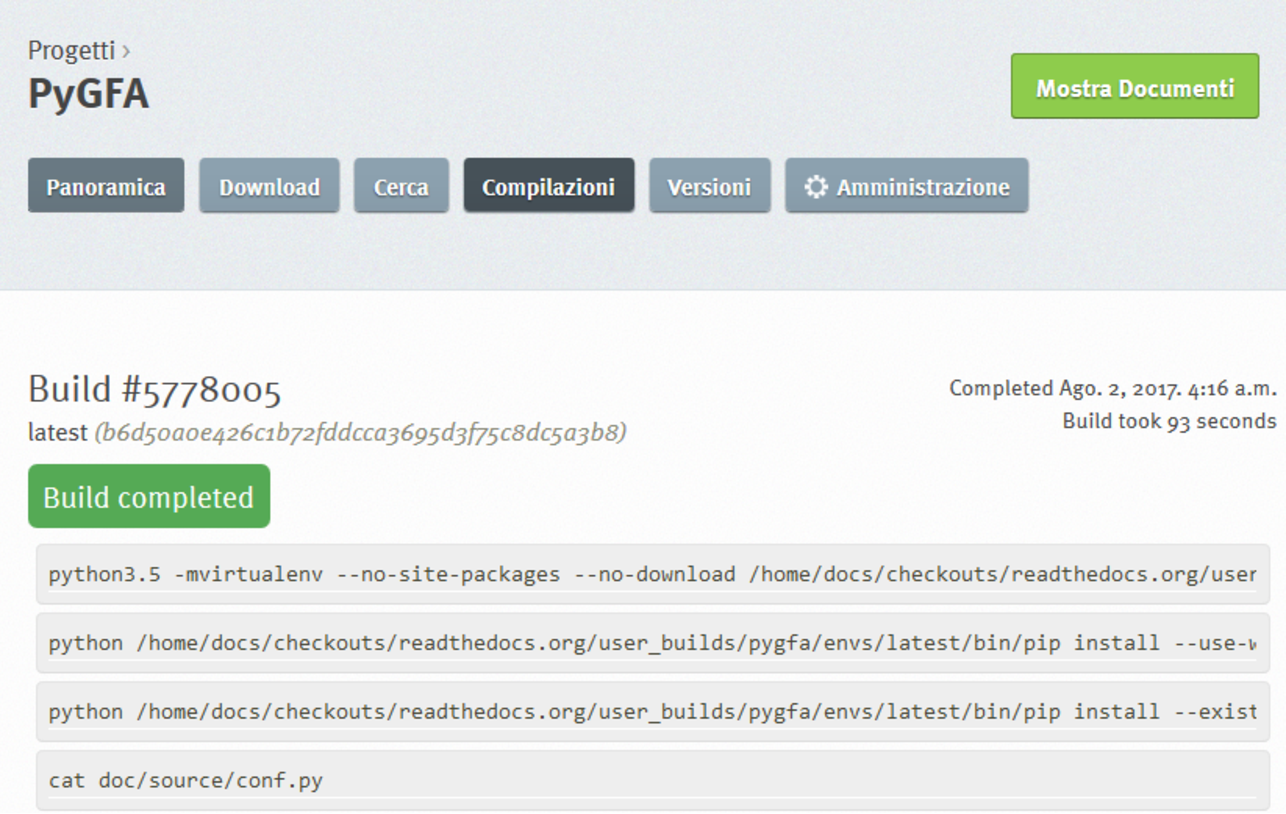
\includegraphics[scale=0.65]{rtd}
	\caption[Schermata di build di Read the Docs.]{Interfaccia per la generazione della documentazione in Read the Docs.}
	\label{fig:rtd-build}
\end{figure}

% git e GitHub
\section{git e GitHub}
\nocite{git}
\emph{git} è un sistema di controllo versione, ideato da Linus Torvalds per
gestire lo sviluppo del kernel Linux, tra i più utilizzati al mondo.
Esso permette di gestire progetti di ogni dimensione, garantendo velocità,
coerenza e ripristino fra le diverse tappe di sviluppo di un progetto.

\begin{wrapfigure} {O} {0.35\textwidth}
	\begin{centering}	
		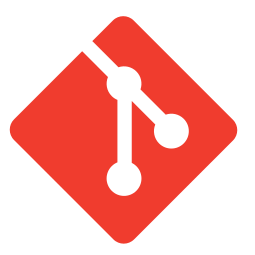
\includegraphics[scale=0.5]{git-logo}
		\caption[Logo git]{Logo dello strumento di controllo versione git.}
	\end{centering}
\end{wrapfigure}

Il programma permette, una volta inizializzato all'interno di una cartella,
di gestire i file in base ai cambiamenti ad essi effettuati. Per integrare
un cambiamento apportato ad un file è necessario aggiungerlo a quella
che viene chiama \emph{staging area}, contenente l'insieme
di file modificati a partire dall'ultimo stato aggiornato del sistema.
Generalmente i file nella staging area sono accomunati da un contesto
comune (una modifica che coinvolge per lo stesso motivo quello specifico
insieme di file), ma ai fini del sistema ciò non è un requisito indispensabile.
Terminate le modifiche e aggiunte alla staging area è necessario integrare
tali modifiche nel sistema mediante una \emph{commit}, un'operazione
che crea un identificativo univoco dello stato del sistema nel momento esatto
in cui i cambiamenti vengono integrati con esso. Grazie alla creazione
di questo identificativo è possibile ritornare nell'esatto stato
del sistema indicato, nel caso fosse necessario.

Git permette non solo di lavorare ad un progetto procedendo in un'unica
sequenza di sviluppo, ma permette la creazione di più diramazioni parallele
(\emph{branch}), indipendenti dalle future modifiche apportate al sistema,
che possono procedere nello sviluppo. Tali diramazioni garantiscono un
ambiente di lavoro isolato e stabile nel quale un singolo sviluppatore può
concentrare il suo sviluppo, senza preoccuparsi delle modifiche che altri
sviluppatori potrebbero apportare al sistema, per poi far ricongiungere
il componente nella principale sequenza di sviluppo (solitamente indicato
dal branch \emph{master}).

La flessibilità di sviluppo che questo strumento offre permette di strutturare
al meglio le diverse fasi di implementazione di un progetto, in piena coerenza con
un processo agile o di extreme programming. In \pygfa tale caratteristica
si è rivelata di fondamentale importanza, permettendo di suddividere
fasi di refactoring o di ridefinizione della struttura di progetto (operazioni
molto delicate da un punto di vista della stabilità della libreria) in un
ambiente controllato e reversibile in caso di problemi.

Completate le modifiche ed effettuata la commit, è possibile sincronizzare
i cambiamenti locali con una repository remota, un luogo decentralizzato
sul quale il lavoro viene salvato e grazie al quale è possibile condividere
il progetto con i propri collaboratori. Una tra le più famose piattaforme
che permettono di ospitare un repository git remoto è \emph{GitHub}.

GitHub è un sito che offre funzionalità paragonabili a quelle che Read
the Docs (vedi sezione \ref{seq:sphinx-rtd} a pagina \pageref{seq:sphinx})
fornisce per Sphinx. Permette di ospitare repository remote, catalogarle
per una maggiore accessibilità (se pubbliche) offrendo un'interfaccia
intuitiva per:
\begin{itemize}
	\item la creazione di \emph{tag} per il rilascio delle versioni stabili del sistema,
	\item la creazione di aree di discussione relative a bachi, miglioramenti e problematiche
		generali, fornendo agli sviluppatori un luogo centralizzato e coerente
		per la discussione di queste tematiche,
	\item lla creazione di punti di branching e analisi delle diverse ramificazioni del sistema
		e dell'attuale sequenza di sviluppo del progetto,
	\item la navigazione dell'intero progetto, con la possibilità di ispezionarlo
		ricreandone lo stato dopo una specifica commit,
	\item la visione di statistiche relative le commit effettuate da chiunque
		abbia contribuito al sistema, con la possibilità di analizzare le modifiche
		apportate a livello di singola commit.
\end{itemize}

Il ruolo che questi due strumenti hanno avuto e avranno nello lo sviluppo
di \pygfa è \emph{incalcolabile}. Non solo ai fini del salvataggio del
progetto, della sua gestione e della sua reperibilità, ma anche per la
possibilità che esso offre di permettere ad un qualsiasi sviluppatore di
effettuare facilmente una diramazione del codice ai fini di poterlo
riscrivere in base alle proprie necessità, senza doversi cimentare
nello sviluppo di un sistema nuovo (\emph{fork}).

% Bandage
\section{Bandage}
\label{sec:bandage}
\nocite{doi:10.1093/bioinformatics/btv383}
Bandage è un programma per la visualizzazione grafica di grafi
di assemblaggio. Questo strumento è in grado di visualizzare
grafi descritti da file GFA1, per questo il suo impiego
è stato di vitale importanza nell'analisi dei collegamenti presenti fra
le sequenze, specialmente nei casi di dovetail overlap, che descrivono
un continuum nel genoma e che per tanto costituiscono un'informazione
di rilievo per una libreria che si occupa della gestione di questi file.

\section{Conclusioni}
In questo capitolo sono stati presentati gli strumenti impiegati nello sviluppo
di \pygfa, nella fase di test e di documentazione indicando i dettagli
che si sono rivelati di particolare importanza ai fini implementativi del sistema.